\documentclass{beamer}

\usetheme{simple}

\newcommand{\emojimoyai}{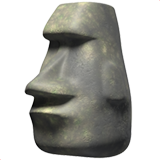
\includegraphics[width=12pt]{img/moyai.png}}

\usepackage{caption}
\usepackage{xcolor}
\usepackage{fancyvrb}
\usepackage{ulem}
\usepackage{subcaption}
\usetikzlibrary{positioning,calc,automata}

\title{CSC363 Tutorial \#5}
\subtitle{``Review'' (and some useful facts for A3?)}
\date{February 16, 2022}
\institute{}

\newcommand{\N}{{\mathbb N}}
\newcommand{\R}{{\mathbb R}}
\newcommand{\inner}[1]{\langle #1 \rangle}

\setwatermark{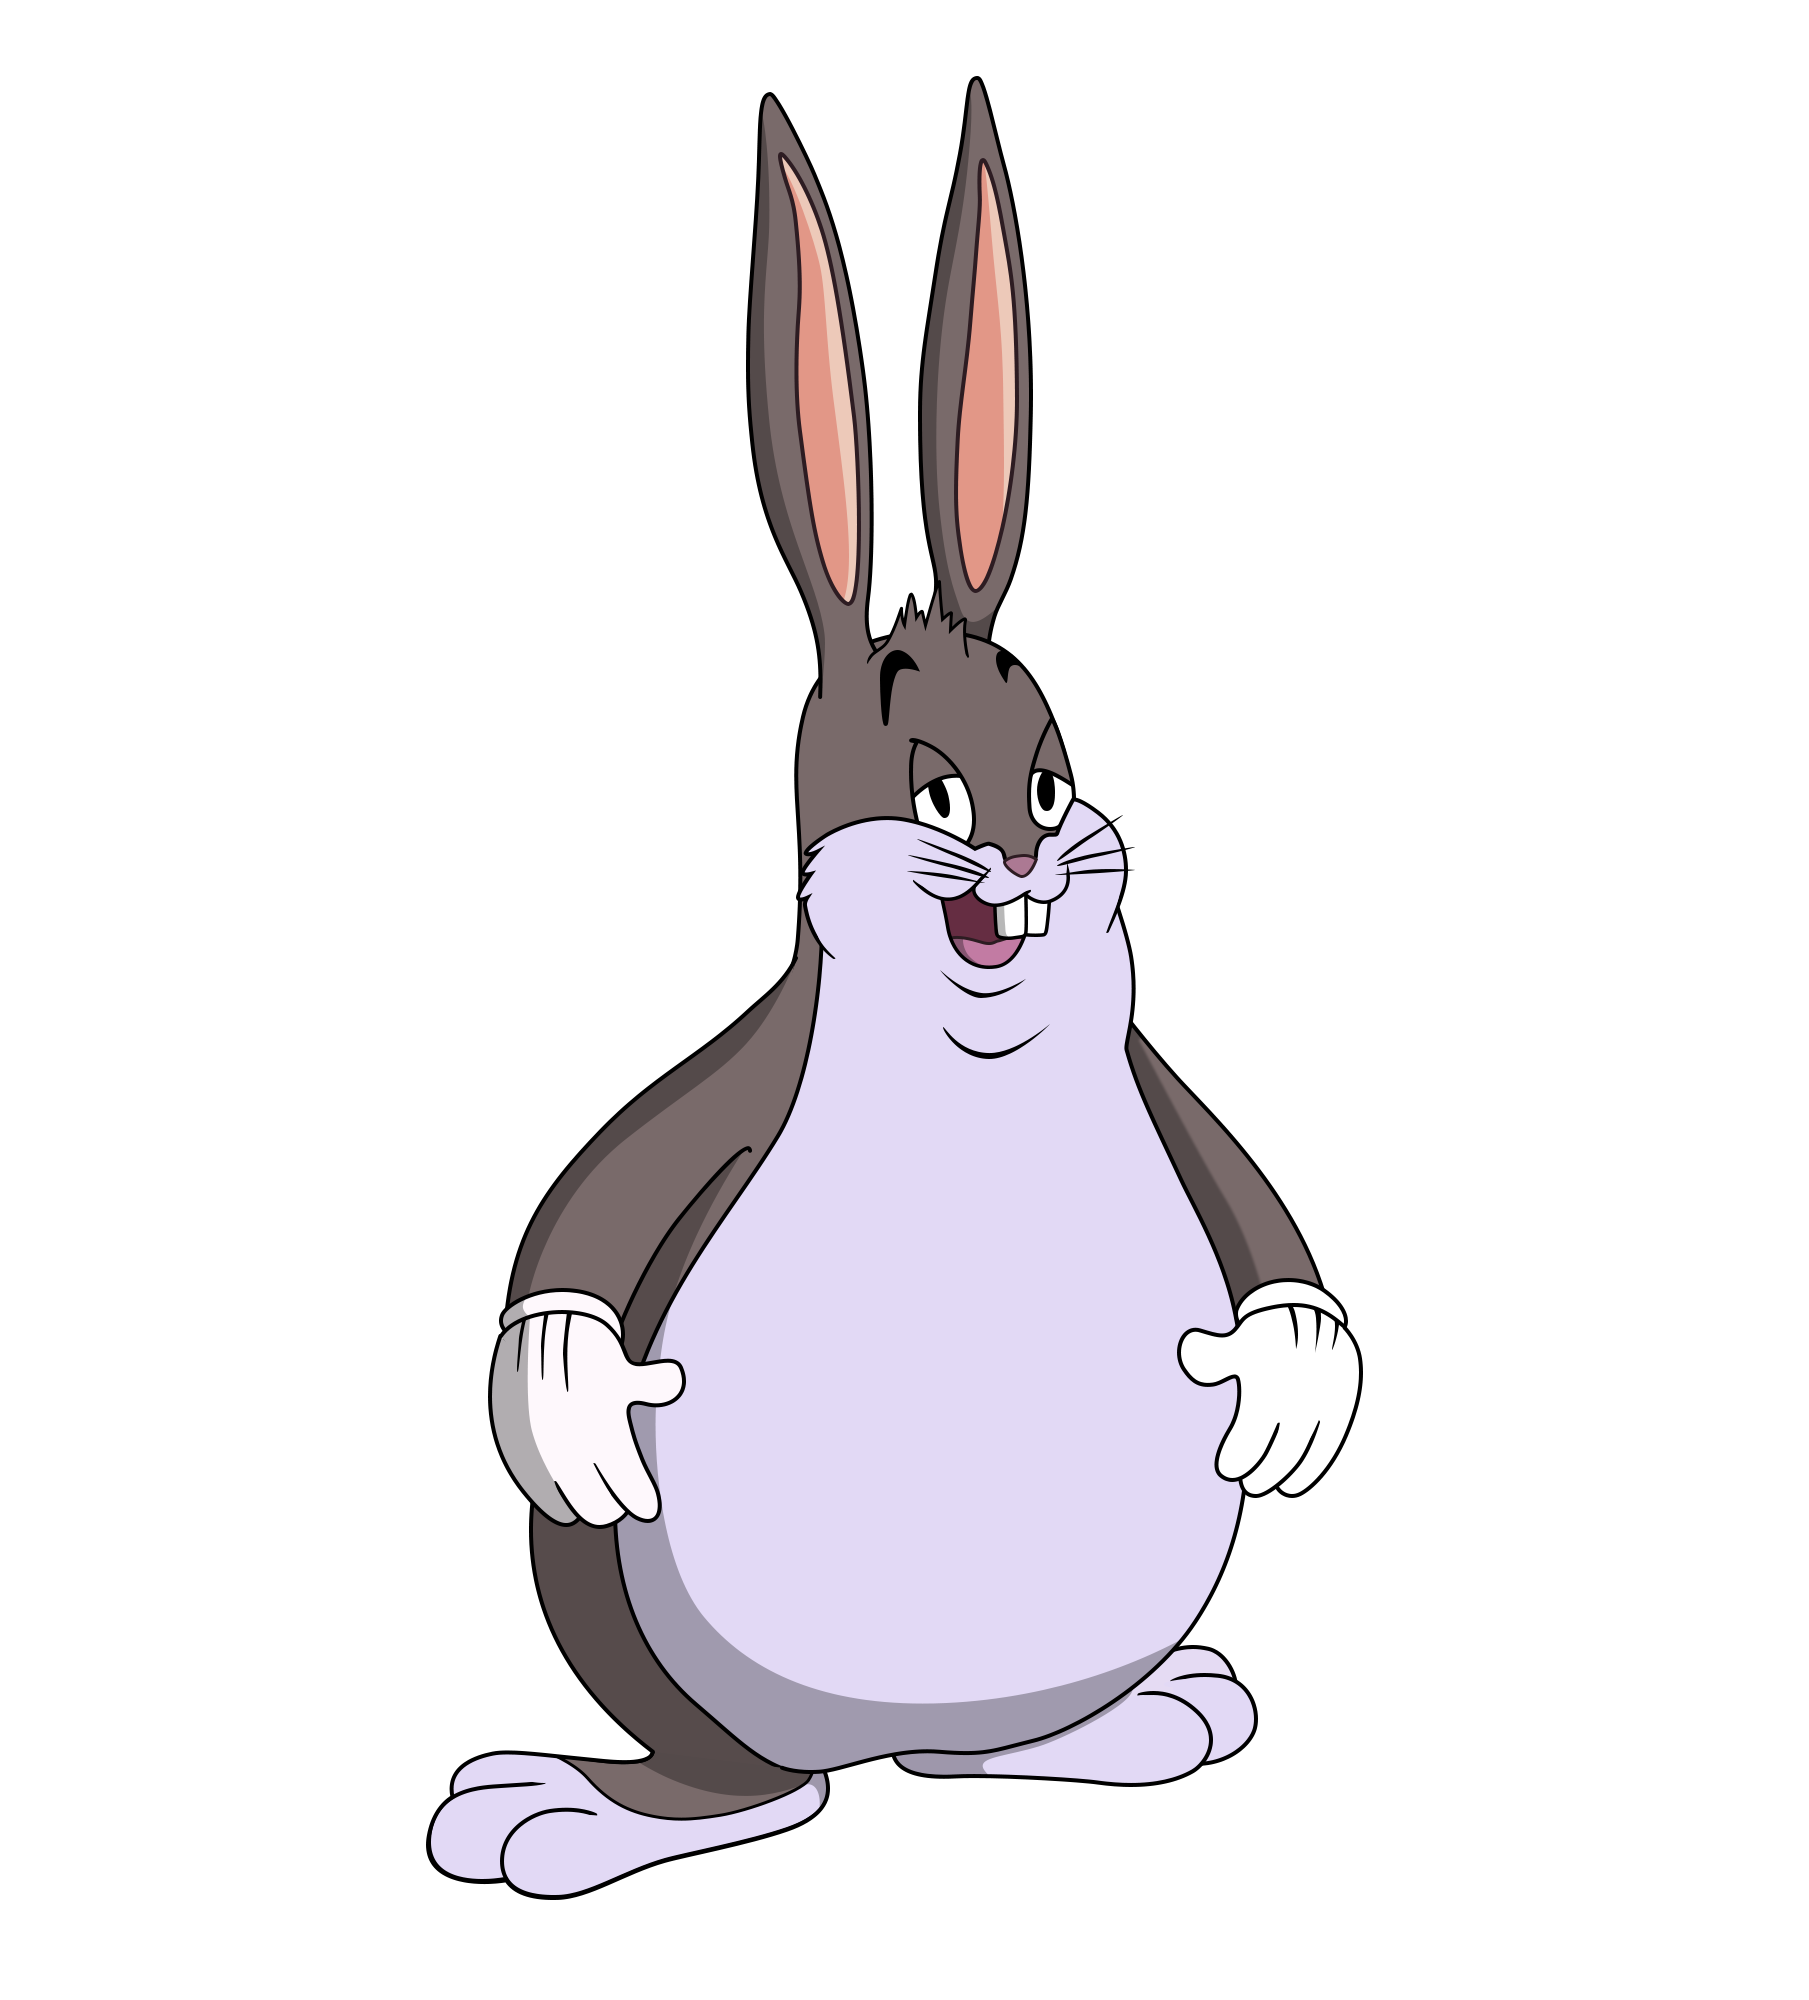
\includegraphics[height=8cm]{img/chungus.png}}

\begin{document}

\maketitle

\begin{frame}{Learning objectives this tutorial}
\begin{itemize}
\item Review $m$-reductions and $1$-reductions.
\item Prove some useful facts that you might need for your assignment...
\item Recall/prove properties of countablility/uncountability.
\item Show that ``busy beaver'' is a non-computable function! (for fun, of course)
\end{itemize}
\end{frame}

\begin{frame}{Stuff from like, the past few weeks}
\textbf{Task:} Categorize these terms describing sets into ``computable'', ``CE'', or ``neither''.
\vspace{2mm}

\begin{center}
\begin{minipage}{0.4\textwidth}
\begin{itemize}
    \item Listable
    \item Diophantine
    \item Countable
    \item Uncountable
    \item Decidable
\end{itemize}
\end{minipage}
\begin{minipage}{0.4\textwidth}
\begin{itemize}
    \item $\Sigma_0$
    \item $\Pi_0$
    \item $\Sigma_1$
    \item $\Pi_1$
    \item $\Sigma_2$
\end{itemize}
\end{minipage}
\end{center}
\end{frame}

\begin{frame}{Stuff from last lecture?}

\textbf{Question:} What is the definition of $A \leq_m B$ and $A \equiv_1 B$?

\pause

\textbf{Ans:} Given two sets $A, B \subseteq \N$, we say that $A \leq_m B$ if there exists a \textit{computable} $f: \N \to \N$ such that
$$x \in A \Leftrightarrow f(x) \in B.$$

\begin{figure}
    \centering
    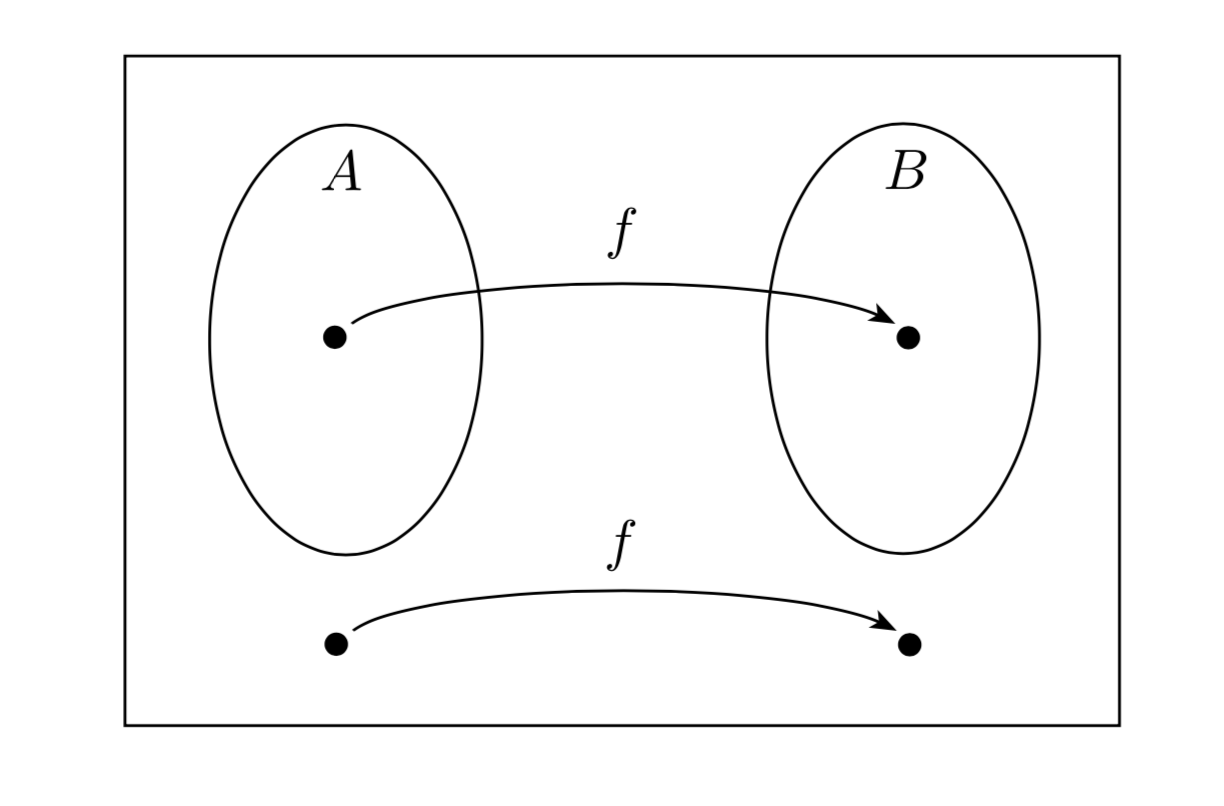
\includegraphics[scale=0.3]{img/mapping_reduc.png}
\end{figure}

If $A \leq_m B$ and $B \leq_m A$, we say that $A \equiv_m B$.

\end{frame}

\begin{frame}{Stuff from last lecture?}

\textbf{Question:} What is the definition of $A \leq_1 B$ and $A \equiv_1 B$?

\pause

\textbf{Ans:} Given two sets $A, B \subseteq \N$, we say that $A \leq_m B$ if there exists a \textit{computable and injective} $f: \N \to \N$ such that
$$x \in A \Leftrightarrow f(x) \in B.$$

If $A \leq_1 B$ and $B \leq_1 A$, we say that $A \equiv_1 B$.

\pause

Immediately from the definitions, $A \leq_1 B \Rightarrow A \leq_m B$. However, the converse $A \leq_m B \Rightarrow A \leq_1 B$ does not hold in general.
\end{frame}

\begin{frame}{Assignment 3 \emojimoyai}

\textbf{Definition:} A set $S \subseteq \N$ is a \textbf{cylinder} if there is a set $B \subseteq \N$ such that
$$S \equiv_1 B \times \N.$$

\textbf{Task:} Show that for any computable set $S$ that isn't $\emptyset$ or $\N$, $S \leq_1 S \times \N$. \pause
\textbf{Ans:} Since $S \neq \emptyset$ and $S \neq \N$, we can find a $p \in S$ and a $q \notin S$. Define
$$f(x) = \begin{cases}
\inner{p, x} & x \in S\\
\inner{q, x} & x \notin S.\\
\end{cases}$$
$f$ is computable and injective. Why? Find out on the next episode.\footnote{Or you may just prove it yourself instead.}

\end{frame}

\begin{frame}{Assignment 3 \emojimoyai}

\textbf{Definition:} A set $S \subseteq \N$ is a \textbf{cylinder} if there is a set $B \subseteq \N$ such that
$$S \equiv_1 B \times \N.$$

\textbf{Task:} Find a set $S$ such that $B \times \N \not \leq_1 S$ for any $B$. \textit{Hint: consider the cardinality of $S$.}

\pause

\textbf{Ans:} Any nonempty finite set $S$ will do, such as $S = \{192168011\}$. Consider any set $B$:\pause
\begin{itemize}
    \item If $B = \emptyset$ then $B \times \N = \emptyset$, but $S$ is nonempty so $B \times \N \not \leq_1 S$ (Why?).\pause
    \item If $B \neq \emptyset$, then $B \times \N$ is infinite (Why?). But $S$ is finite, so there is no way to create an injection from $B \times \N$ to $S$, which means $B \times \N \not \leq_1 S$.
\end{itemize}
\pause
\textbf{Question:} We've found a set $S$ such that $S \times \N \not \leq_1 S$. Is it necessarily true that for any set $S$, $S \times \N \leq_m S$? \pause 

\textbf{Ans:} Yes (consider the function $f\inner{s, n} = s$).
\end{frame}

\begin{frame}{Speaking of cardinality...}
Hope you remember your MAT102 stuff!

\pause

\textbf{Definition:} A set $S$ (not necessarily a subset of the naturals) is \textbf{countable} if there is an injection from $S$ to $\N$ (or in other words, $|S| \leq |\N|$).

\pause

\textbf{Note:} ``Countable'' in this course includes finite!

\textbf{Task:} Categorize the following sets into ``countable'' and ``uncountable''.

\begin{minipage}{0.3\textwidth}
\begin{itemize}
    \item $\N$
    \item $\R$
    \item $\N \times \N$
    \item $\mathbb Q$
    \item $\N^n$
    \item $P(\N)$ (power set)
\end{itemize}
\end{minipage}
\begin{minipage}{0.6\textwidth}
\begin{itemize}
    \item The set of functions from $\N$ to $\N$
    \item The set of computable functions from $\N$ to $\N$
    \item The set of all possible computer programs in ASCII
    \item The set of objects Big Chungus has consumed over the last 24 hours
\end{itemize}
\end{minipage}
\end{frame}

\begin{frame}{Speaking of cardinality...}
Hope you remember your MAT102 stuff!

\pause

\textbf{Definition:} A set $S$ (not necessarily a subset of the naturals) is \textbf{countable} if there is an injection from $S$ to $\N$ (or in other words, $|S| \leq |\N|$).

\pause

\textbf{Task:} Let $S_0, S_1, \ldots$ be a countably infinite collection of countably infinite and pairwise disjoint sets. Show that
$$\bigcup_{i = 0}^\infty S_i = \{s: \text{$s \in S_i$ for some $i \in \N$}\}$$
is countable.

\textbf{Ans:} Write it out! Let $S_1 = \{s_{11}, s_{12}, \ldots\}$, $S_2 = \{s_{21}, s_{22}, \ldots\}$ and so on. We can then define the injection 
$$f: \bigcup_{i = 0}^\infty S_i \to \N \times \N, f(s_{ij}) = (i, j).$$
This is well-defined and injective, as the $S_i$'s are all disjoint. But we know $\N \times \N$ is countable already!
\end{frame}

\begin{frame}{BusyBeaver}
\begin{figure}
\centering
\begin{subfigure}{0.45\textwidth}
    \centering
    
\includegraphics[width=5cm]{img/busybeaver.png}
\end{subfigure}
\begin{subfigure}{0.45\textwidth}
    \centering
    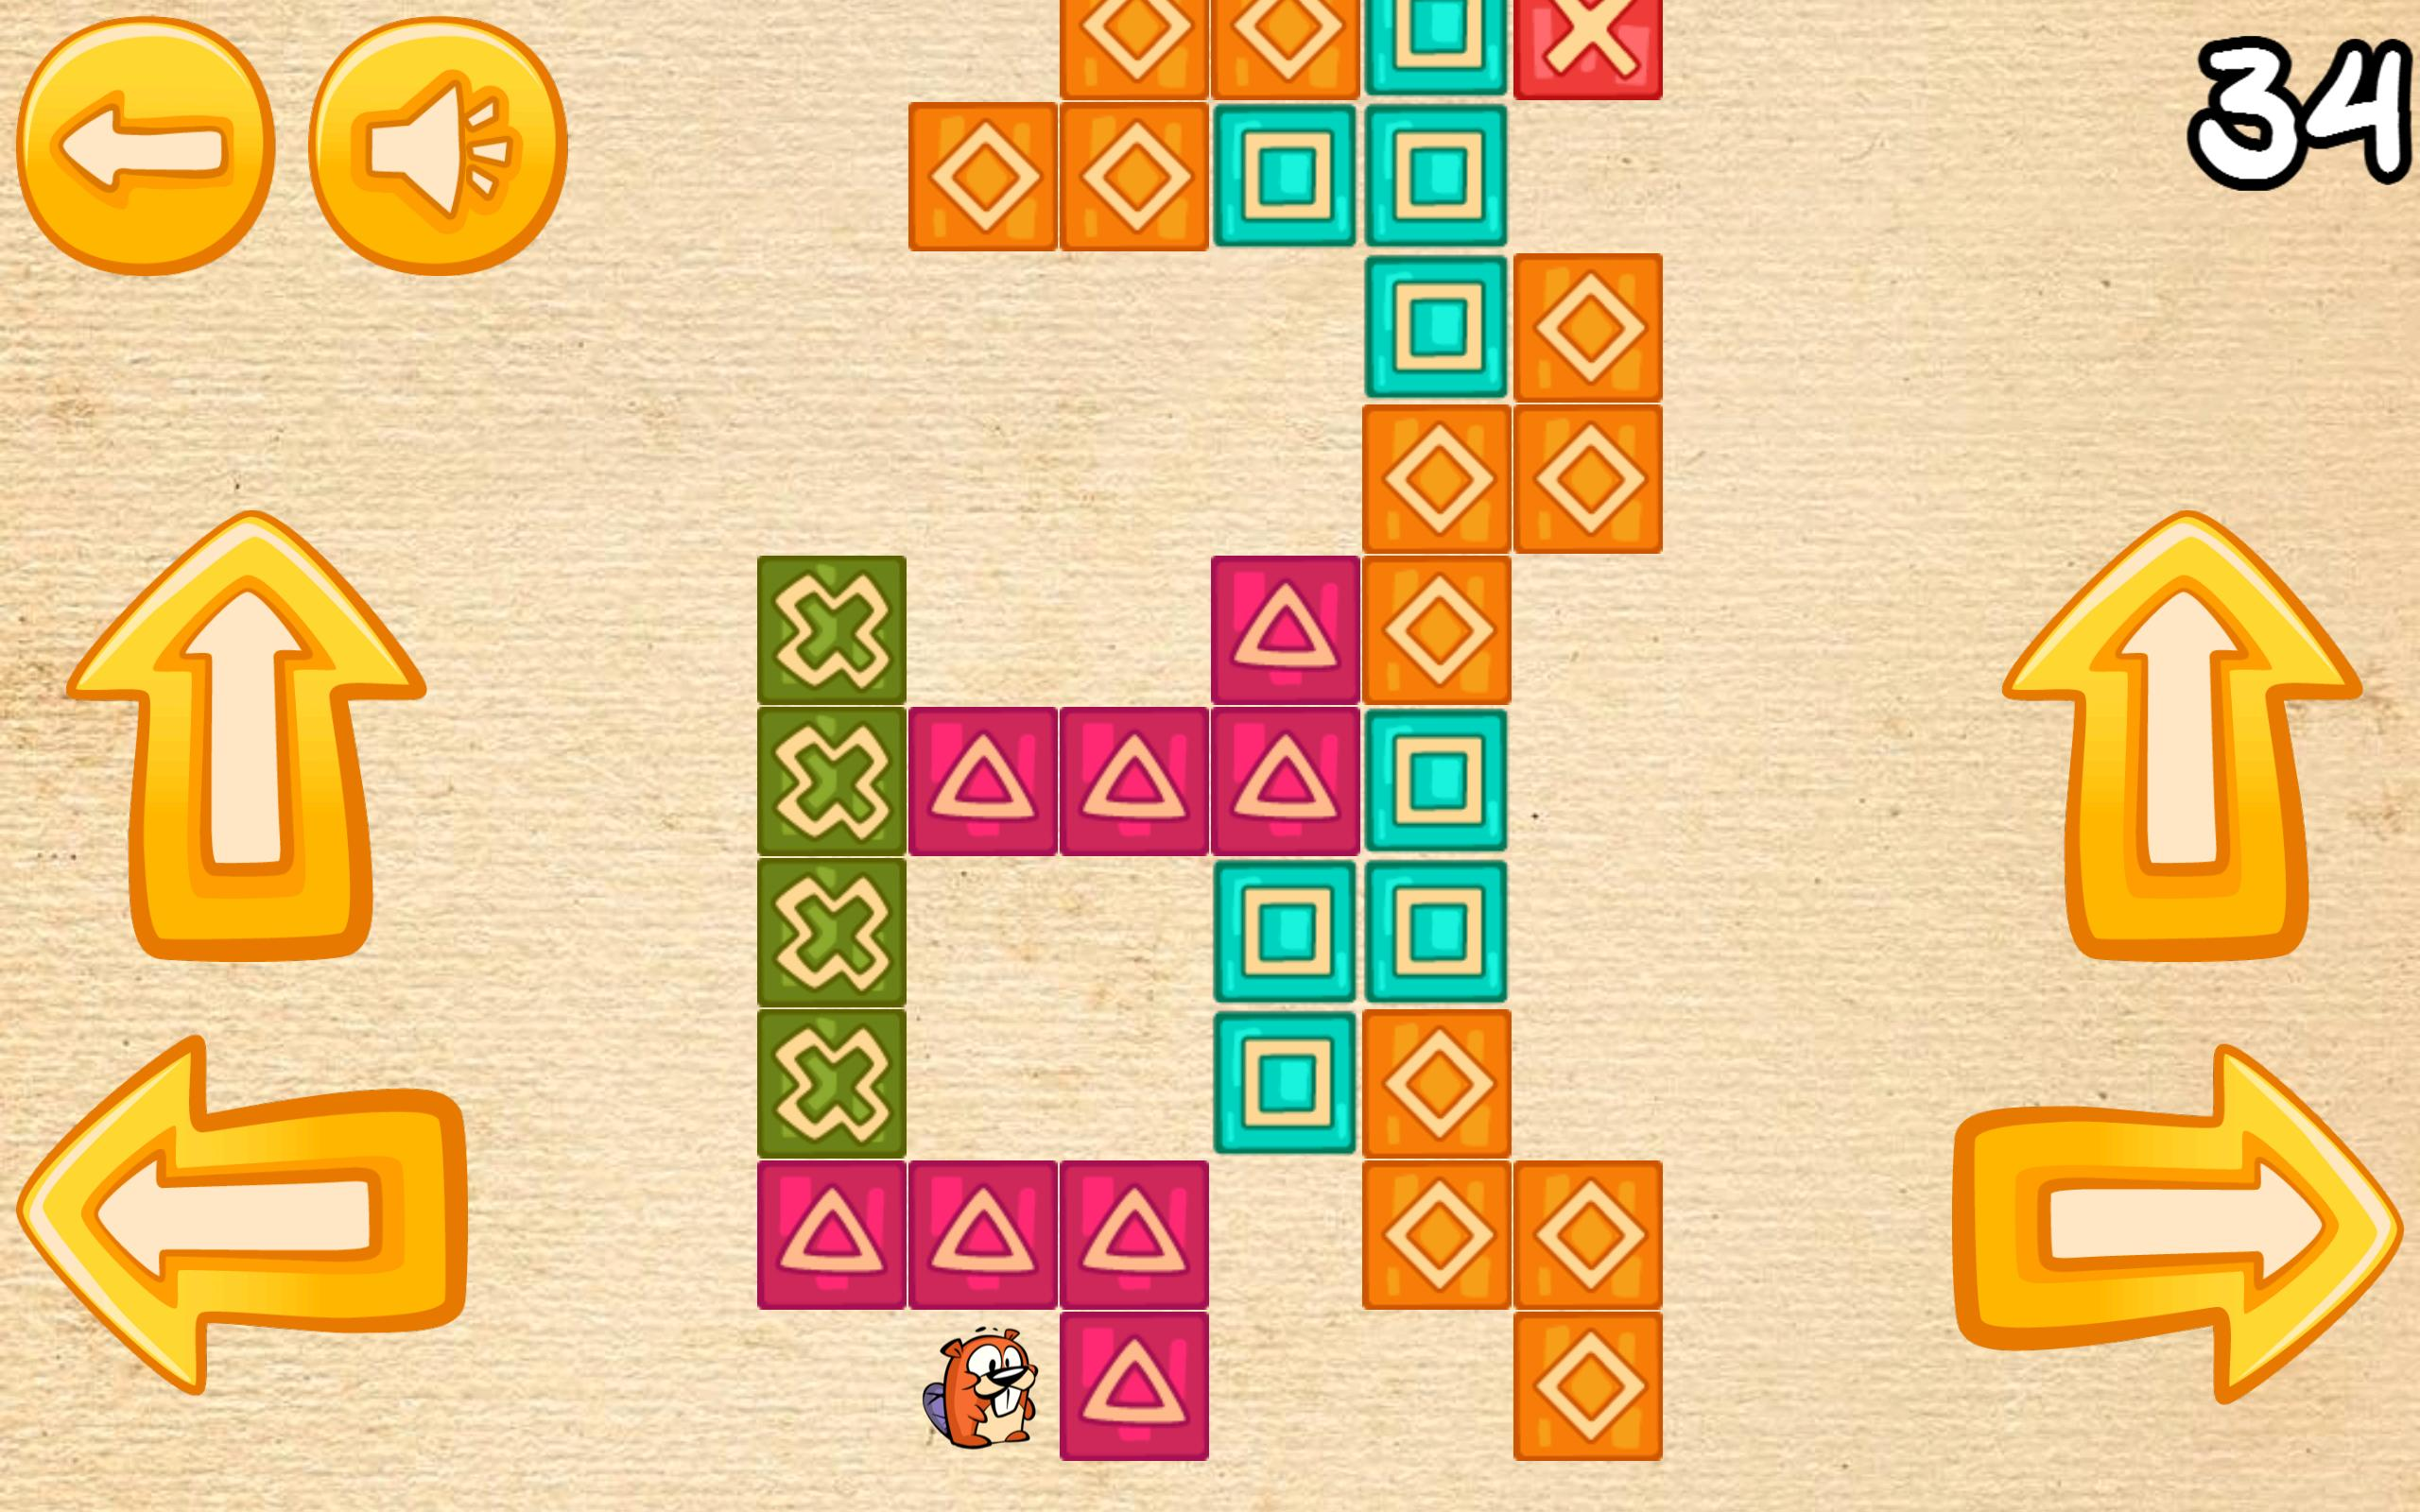
\includegraphics[width=5cm]{img/gameplay.jpg}
\end{subfigure}
    \caption*{Not to be confused with the Android game \textit{Busy Beaver}...}
\end{figure}
Here's the BusyBeaver(n) game!
\begin{quote}
    Design a Turing machine with tape alphabet $\{\square, 1\}$ ($\square$ being the blank symbol), with \textbf{exactly $n$ states} excluding the halting state. This Turing machine \textbf{must halt} with the empty string as input (starting will all $\square$ on the tape). Write as many `1' symbols as you can to the tape, before halting.
\end{quote}
\end{frame}

\begin{frame}{BusyBeaver}
Here's the BusyBeaver(n) game! (for fun only, not needed for this course)
\begin{quote}
    Design a Turing machine with tape alphabet $\{\square, 1\}$ ($\square$ being the blank symbol), with \textbf{exactly $n$ states} excluding the halting state. This Turing machine \textbf{must halt} with the empty string as input (starting will all $\square$ on the tape). Write as many `1' symbols as you can to the tape, before halting.
\end{quote}

\textbf{Task:} Play BusyBeaver(1). That is, build a 1-state (excluding the halting state) TM that writes as many `1's to the tape as possible before halting.

\pause

\textbf{Ans:} There isn't much we can do... the best possible score is one `1' symbol.
\begin{center}
    \begin{tabular}{c|c|c}
        State & Symbol & (newState, newSymbol, dir) \\
        \hline
        start & $\square$ & (halt, $1$, $R$)\\
        start & $1$ & -\\
        halt & - & -
    \end{tabular}
\end{center}
\end{frame}


\begin{frame}{BusyBeaver}
Here's the BusyBeaver(n) game!
\begin{quote}
    Design a Turing machine with tape alphabet $\{\square, 1\}$ ($\square$ being the blank symbol), with \textbf{exactly $n$ states} excluding the halting state. This Turing machine \textbf{must halt} with the empty string as input (starting will all $\square$ on the tape). Write as many `1' symbols as you can to the tape, before halting.
\end{quote}

\textbf{Task:} Play BusyBeaver(2). That is, build a 2-state (excluding the halting state) TM that writes as many `1's to the tape as possible before halting.

\pause

\textbf{Ans:} The best possible score is $4$.
\begin{center}
    \begin{tabular}{c|c|c}
        State & Symbol & (newState, newSymbol, dir) \\
        \hline
        start & $\square$ & ($q_1$, $1$, $R$)\\
        start & $1$ & ($q_1$, $1$, $L$)\\
        $q_1$ & $\square$ & ($q_0$, $1$, $L$)\\
        $q_1$ & $1$ & (halt, $1$, $R$)\\
        halt & - & -
    \end{tabular}
\end{center}
\end{frame}

\begin{frame}{BusyBeaver}
Here's the BusyBeaver(n) game!
\begin{quote}
    Design a Turing machine with tape alphabet $\{\square, 1\}$ ($\square$ being the blank symbol), with \textbf{exactly $n$ states} excluding the halting state. This Turing machine \textbf{must halt} with the empty string as input (starting will all $\square$ on the tape). Write as many `1' symbols as you can to the tape, before halting.
\end{quote}

\textbf{Task:} Play BusyBeaver(6). That is, build a 6-state (excluding the halting state) TM that writes as many `1's to the tape as possible before halting.

\pause

\textbf{Ans:} We actually don't know the best possible score here, but someone came up with a $6$-state TM that can produce $3.515 \times 10^{36534}$ `1's.
\end{frame}

\begin{frame}{BusyBeaver}
Here's the BusyBeaver(n) game!
\begin{quote}
    Design a Turing machine with tape alphabet $\{\square, 1\}$ ($\square$ being the blank symbol), with \textbf{exactly $n$ states} excluding the halting state. This Turing machine \textbf{must halt} with the empty string as input (starting will all $\square$ on the tape). Write as many `1' symbols as you can to the tape, before halting.
\end{quote}

Of course, we can define the \textbf{Busy Beaver Function} $\mathrm{BB}(n)$ as follows:
$$\mathrm{BB}(n) = \text{Best possible score in the BusyBeaver(n) game}.$$
For each $n \in \N$, there are only finitely many $n$-state TMs, so the maximum possible score exists.
\end{frame}

\begin{frame}[fragile]{BusyBeaver}
\textbf{Task:} Prove that $BB(n)$ is not a computable function. That is, there is no program that can compute $BB(n)$ for all $n \in \N$. (Hard!)

\pause

\textbf{Ans:} Suppose there were such a program \texttt{compute\_bb(n)}, towards a contradiction. Build the following program UTM:

\begin{verbatim}
UTM(e, x):
  Create two tapes tape1 and tape2.
  While True:
    On tape1:
      Run one step of the eth turing machine on x. 
    On tape2, write a 1.
    If the eth TM halted, erase tape1, and return.
\end{verbatim}

We can build a Turing machine that runs UTM, say with $k$ states. But then we can write the following program:
\begin{verbatim}
H(e, x):
  max_steps = compute_bb(k)
  Run UTM(e, x) while the # of 1s on tape2 < max_steps.
  If it halts, return True. Else, return False.
\end{verbatim}

\end{frame}

\begin{frame}[fragile]{BusyBeaver}
\textbf{Ans:} Suppose there were such a program \texttt{compute\_bb(n)}, towards a contradiction. Build the following program UTM:

\begin{verbatim}
UTM(e, x):
  Create two tapes tape1 and tape2.
  While True:
    On tape1:
      Run one step of the eth turing machine on x. 
    On tape2, write a 1.
    If the eth TM halted, erase tape1, and return.
\end{verbatim}

We can build a Turing machine that runs UTM, say with $k$ states. But then we can write the following program:
\begin{verbatim}
H(e, x):
  max_steps = compute_bb(k)
  Run UTM(e, x) while the # of 1s on tape2 < max_steps.
  If it halts, return True. Else, return False.
\end{verbatim}

\textbf{Task:} Spot the contradiction. \pause \textbf{Ans:} $H$ solves the halting problem!

\end{frame}


\begin{frame}{BusyBeaver}

Some video on BusyBeaver by Computerphile:
\url{https://www.youtube.com/watch?v=CE8UhcyJS0I}

\begin{figure}
    \centering
    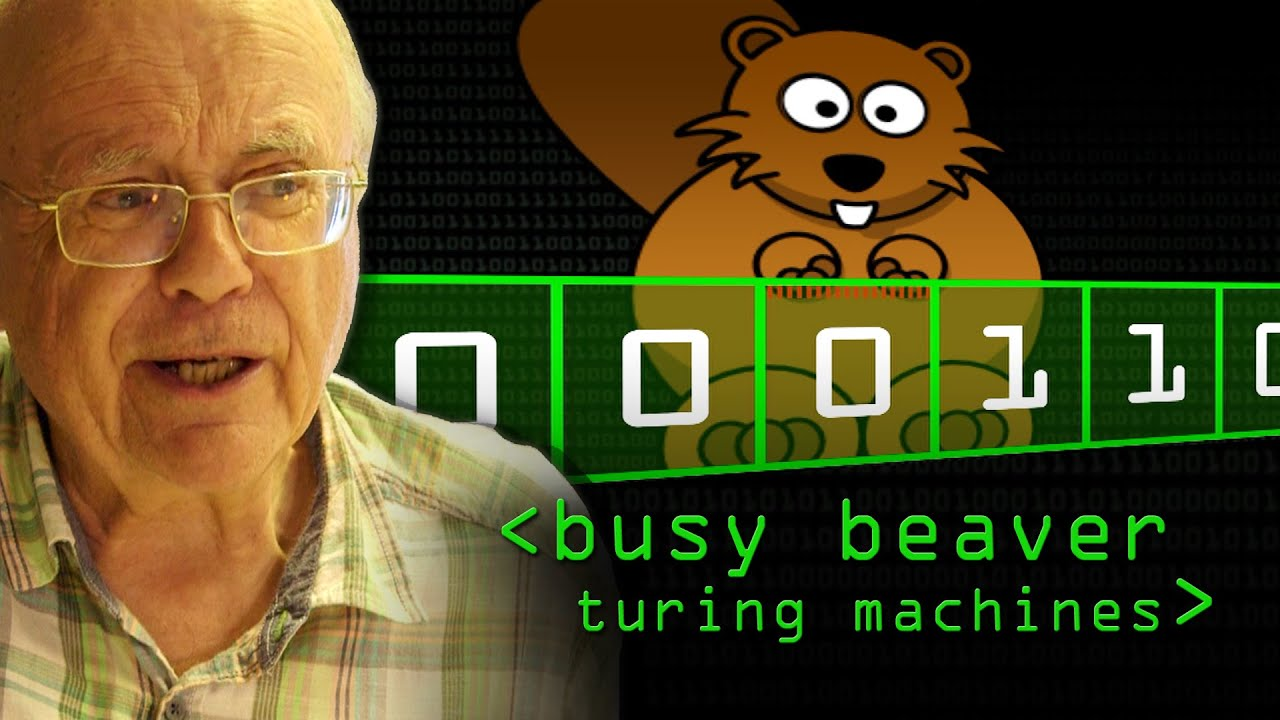
\includegraphics[width=10cm]{img/computerphile.jpg}
    \caption*{You get to listen to this guy talk about BB!}
\end{figure}

\end{frame}





\end{document}